% fig_system_standalone.tex — PixCell pipeline diagram (Fig. 1, fig:system)
% Build: tectonic fig_system_standalone.tex
% Style: serif (Latin Modern), black/gray line work, single muted blue accent.
\documentclass[border=6pt]{standalone}
\usepackage{lmodern}
\usepackage[T1]{fontenc}
\usepackage{tikz}
\usetikzlibrary{arrows.meta, positioning, calc}

\definecolor{accent}{RGB}{60,126,193}% desaturated blue

\begin{document}
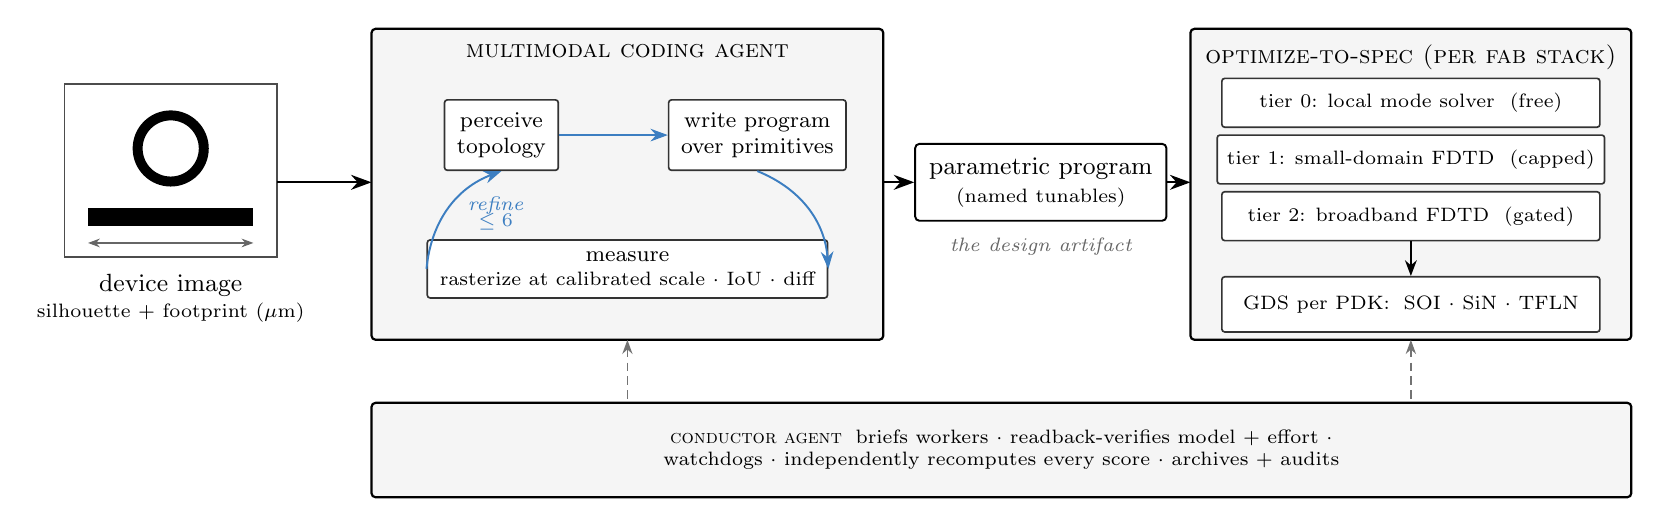
\begin{tikzpicture}[
  every node/.style={font=\small},
  box/.style={draw=black, line width=0.7pt, rounded corners=1.5pt, fill=white,
              inner sep=5pt, align=center},
  innerbox/.style={draw=black!80, line width=0.6pt, rounded corners=1pt, fill=white,
                   inner sep=4.5pt, align=center, font=\footnotesize},
  group/.style={draw=black, line width=0.8pt, rounded corners=1.5pt, fill=gray!8},
  tier/.style={draw=black!80, line width=0.6pt, rounded corners=1pt, fill=white,
               inner sep=3.5pt, align=center, font=\scriptsize, minimum width=48mm,
               minimum height=6.2mm},
  flow/.style={-{Stealth[length=2.6mm, width=1.9mm]}, line width=0.8pt},
  loop/.style={-{Stealth[length=2.2mm, width=1.6mm]}, line width=0.7pt, accent},
  cond/.style={densely dashed, line width=0.5pt, black!55},
  gtitle/.style={font=\small\scshape},
  note/.style={font=\scriptsize\itshape, text=black!60},
]

% =========================== input: device image ===========================
% image frame
\draw[black!70, line width=0.6pt, fill=white] (-1.35,-0.10) rectangle (1.35,2.10);
% silhouette: bus waveguide + ring
\fill[black] (-1.05,0.30) rectangle (1.05,0.52);
\draw[black, line width=3.6pt] (0,1.28) circle (0.42);
% footprint dimension line
\draw[{Stealth[length=1.5mm,width=1.1mm]}-{Stealth[length=1.5mm,width=1.1mm]},
      line width=0.4pt, black!60] (-1.05,0.08) -- (1.05,0.08);
\node[align=center] at (0,-0.62)
  {device image\\[-1.5pt] {\scriptsize silhouette $+$ footprint ($\mu$m)}};

% ====================== stage 1: multimodal coding agent ======================
\draw[group] (2.55,-1.15) rectangle (9.05,2.80);
\node[gtitle, anchor=north] at (5.80,2.72) {multimodal coding agent};

\node[innerbox] (perceive) at (4.20,1.45) {perceive\\topology};
\node[innerbox] (write)    at (7.45,1.45) {write program\\over primitives};
\node[innerbox] (measure)  at (5.80,-0.25)
  {measure\\[-1pt]{\scriptsize rasterize at calibrated scale $\cdot$ IoU $\cdot$ diff}};

\draw[loop] (perceive.east) -- (write.west);
\draw[loop] (write.south) to[bend left=32] (measure.east);
\draw[loop] (measure.west) to[bend left=32]
  node[pos=0.45, right=4.5pt, font=\scriptsize\itshape, text=accent, align=center]
  {refine\\[-2pt]$\leq 6$} (perceive.south);

% ========================= artifact: parametric program =========================
\node[box] (program) at (11.05,0.85)
  {parametric program\\[-1pt]{\scriptsize (named tunables)}};
\node[note, below=2.5pt of program] {the design artifact};

% ===================== stage 2: optimize-to-spec (tiered physics) =====================
\draw[group] (12.95,-1.15) rectangle (18.55,2.80);
\node[gtitle, anchor=north] at (15.75,2.72) {optimize-to-spec (per fab stack)};

\node[tier] (t0) at (15.75,1.86) {tier 0: local mode solver \ (free)};
\node[tier] (t1) at (15.75,1.14) {tier 1: small-domain FDTD \ (capped)};
\node[tier] (t2) at (15.75,0.42) {tier 2: broadband FDTD \ (gated)};

\node[tier, minimum height=7mm] (gds) at (15.75,-0.70)
  {GDS per PDK:\; SOI $\cdot$ SiN $\cdot$ TFLN};
\draw[-{Stealth[length=2.0mm, width=1.5mm]}, line width=0.7pt]
  (t2.south) -- (gds.north);

% ================================ main flow ================================
\draw[flow] (1.35,0.85) -- (2.55,0.85);
\draw[flow] (9.05,0.85) -- (program.west);
\draw[flow] (program.east) -- (12.95,0.85);

% =============================== conductor ===============================
\draw[group] (2.55,-3.15) rectangle (18.55,-1.95);
\node[align=center, font=\scriptsize, text width=148mm] at (10.55,-2.55)
  {{\scshape conductor agent}\; briefs workers $\cdot$ readback-verifies
   model $+$ effort $\cdot$ watchdogs $\cdot$ independently recomputes
   every score $\cdot$ archives $+$ audits};

\draw[cond, {Stealth[length=1.8mm,width=1.3mm]}-] (5.80,-1.15) -- (5.80,-1.95);
\draw[cond, {Stealth[length=1.8mm,width=1.3mm]}-] (15.75,-1.15) -- (15.75,-1.95);

\end{tikzpicture}
\end{document}
